\chapter{光子軌道、リンドラー空間、シュヴァルツシルト内部}

ニュートン的な点質量とシュヴァルツシルトブラックホールは、同じ理想化から出発する。すなわち、重力を及ぼす質量のすべてが中心に集中しているという理想化である。それにもかかわらず、両者の中心の意味は大きく異なる。ニュートン力学では、わずかでも角運動量をもつ粒子は中心を外れる。ブラックホールでは、粒子が事象の地平面を一度越えてしまえば、特異点を外れることはできない。この違いを理解するために、円軌道、光子球、そして最終的には地平面近傍の新しい座標系を順に見ていくことになる。

\section{外れることのできない中心}

現実のニュートン的な物質が数学的な点になることは決してない。圧力、物質の強度、その他の力が圧縮に抵抗する。それでもなお点質量を理想化として用いるとしても、落下する粒子がそれに衝突することはほとんどない。完全に動径方向の軌道ならば\(r=0\)に到達しうるが、わずかな横方向の速度でも角運動量を与える。すると遠心力の障壁が粒子を中心の周りで反転させる。

一般相対性理論はこの結論を変える。十分にコンパクトな天体はブラックホールを形成しうるし、ブラックホール内部では、中心を迂回することによってニュートン的な脱出が打ち破られる。その理由は、単に力が強いということよりも深い。地平面の内側では、\(r\)が減少することは未来の方向なのである。この主張には、仮定するのではなく、徐々に到達することになる。

\begin{classroomqa}
\audiencequestion{中心に衝突することがニュートン力学で難しいのは、単に両方の対象を点として扱っていることの帰結にすぎないのだろうか。}
\lecturerresponse{点という理想化はこの比較の一部ではあるが、区別のすべてではない。ニュートン力学では、ゼロでない角運動量があれば、軌道はその点の周りを通り過ぎる。相対論的な内部では、特異点は落下するすべての時間的軌道の未来に位置しており、角運動は脱出の手段を与えない。
\lecturetimestamp{00:04:52--00:05:13}}
\end{classroomqa}

\section{地平面と特異点}

ここでは当面、シュヴァルツシルト幾何学を所与のものとして受け取る。
\begin{equation}
d\tau^{2}
=
\left(1-\frac{2MG}{r}\right)dt^{2}
-
\frac{dr^{2}}{1-\frac{2MG}{r}}
-
r^{2}d\Omega^{2}.
\label{eq:l6-schwarzschild}
\end{equation}
この計量を選び出す場の方程式は後で扱う。当面の課題は、この計量が何を述べているかを学ぶことである。

単位球面上の計量は、\(\vartheta\)が赤道面から測った緯度であるとき、
\begin{equation}
d\Omega^{2}
=d\vartheta^{2}+\cos^{2}\vartheta\,d\phi^{2}
\label{eq:l6-angular-metric}
\end{equation}
と書くことができる。軸から測るより通常の極角を用いれば、余弦は正弦になる。球対称性により、すべての軌道を一つの固定した平面内に置くことができるので、以下の計算では角座標は一つだけが残ることになる。

\begin{figure}[htbp]
\centering
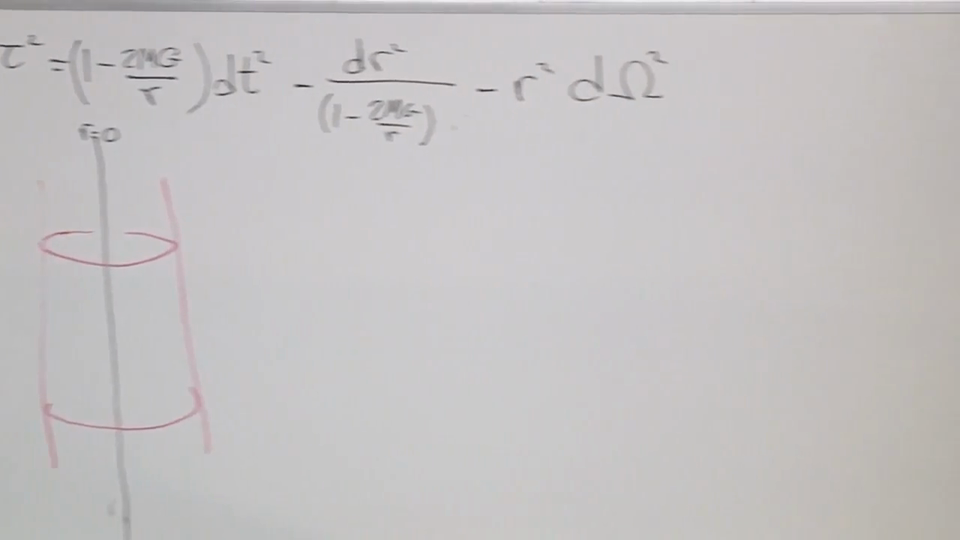
\includegraphics[width=0.88\textwidth]{lecture_06_figure_01.png}
\caption{シュヴァルツシルト計量と、曲面\(r=2MG\)の円筒時空描像。中心の線が\(r=0\)であり、赤い円筒がシュヴァルツシルト座標における地平面である。}
\lectureframe{00:09:45}
\end{figure}

光源から遠く離れると、\(2MG/r\)は小さくなり、式~\eqref{eq:l6-schwarzschild}は球座標におけるミンコフスキー計量に近づく。際立つ半径が二つある。
\begin{equation}
r=2MG,
\qquad
r=0.
\end{equation}
これらを混同してはならない。\(r=2MG\)では、\(dt^{2}\)の係数が消え、\(dr^{2}\)の係数が発散する。シュヴァルツシルト座標系が特異になっているのである。曲率自体はそこでも有限のままである。これに対して\(r=0\)では、曲率不変量が発散する。潮汐場は広がりをもつ物体を動径方向に引き伸ばし、横方向に際限なく圧縮する。これは座標の欠陥ではなく、物理的な特異点である。

\subsection{落下を計時する二つの方法}

地平面の外側にある静止した時計に対しては、
\begin{equation}
d\tau
=
\sqrt{1-\frac{2MG}{r}}\,dt.
\label{eq:l6-static-clock}
\end{equation}
\(r\)が大きいとき、\(d\tau\simeq dt\)である。地平面の近くでは、固定した\(r\)に保たれた時計の固有時は、遠方で保たれるシュヴァルツシルト時間に対して非常にゆっくりと進む。

同じ座標系では、動径方向の落下が\(r=2MG\)に到達するのに\(t\)の無限の値を要するものとして記述される。落下する者自身の経過固有時は有限である。これらの記述の間に矛盾はない。落下する者が携帯する時計は、その世界線に沿った固有時を測る。それは機械式時計であっても、物差しの両端の鏡で作られた光時計であっても、心拍であっても、脳内の物理的過程の連なりであってもよい。これらのいずれも、遠方の座標\(t\)を測ってはいない。この二つの時計の区別は、地平面近傍の図において可視化されることになる。

\section{固有時作用からの円運動}

落下運動に戻る前に、別の問題を解いておこう。どのような条件の下で、質量を持つ粒子や光子がブラックホールの周りを周回できるのだろうか。計算は、自由に運動する任意の相対論的粒子に用いるのと同じ作用原理から始まる。
\begin{equation}
S=-m\int d\tau.
\label{eq:l6-particle-action}
\end{equation}
光は地球によって曲げられるが、地球の重力場は光線を閉じた軌道にするにはまったく十分な強さではない。地球のシュヴァルツシルト半径はわずか1センチメートル程度である。強重力場の問題が関係してくる前に、地球全体をほぼその尺度、すなわち小さな木の実ほどの大きさに圧縮しなければならないだろう。

\(c=1\)とし、運動を赤道面に制限し、
\begin{equation}
F(r)=1-\frac{2MG}{r},
\qquad
G(r)=\frac{1}{F(r)}.
\label{eq:l6-fg}
\end{equation}
と定義する。座標時間\(t\)をパラメータとして用いると、
\begin{equation}
d\tau
=dt\sqrt{F-G\dot r^{\,2}-r^{2}\dot\theta^{\,2}},
\end{equation}
となり、したがって
\begin{equation}
\mathcal L
=
-m\sqrt{F-G\dot r^{\,2}-r^{2}\dot\theta^{\,2}}.
\label{eq:l6-lagrangian}
\end{equation}
となる。因子\(m\)は作用に通常の次元、すなわちエネルギー×時間を与える。

\begin{figure}[htbp]
\centering
\includegraphics[width=0.76\textwidth]{lecture_06_figure_02.png}
\caption{黒板に組み立てられつつある平方根型粒子ラグランジアン。完全な表式は式~\eqref{eq:l6-lagrangian}に与えられている。}
\lectureframe{00:31:53}
\end{figure}

任意の一般化座標\(q\)に対して、
\begin{equation}
p_q=\frac{\partial\mathcal L}{\partial\dot q}.
\end{equation}
ラグランジアンには\(\mathcal L\)を、角運動量には\(L\)を割り当てておくと便利である。
\begin{equation}
\Delta=F-G\dot r^{\,2}-r^{2}\dot\theta^{\,2},
\end{equation}
とすると、二つの運動量は
\begin{align}
L=p_\theta
&=\frac{mr^{2}\dot\theta}{\sqrt{\Delta}},
\label{eq:l6-angular-momentum}\\
p_r
&=\frac{mG\dot r}{\sqrt{\Delta}}.
\label{eq:l6-radial-momentum}
\end{align}
である。動径座標がラグランジアンに現れるため、動径運動量は保存されない。角度\(\theta\)は現れないので、\(L\)は保存される。

\(\mathcal L\)には\(t\)も陽に現れない。したがってハミルトニアンは保存される。
\begin{align}
E=H
&=p_r\dot r+L\dot\theta-\mathcal L \\
&=\frac{mG\dot r^{\,2}}{\sqrt{\Delta}}
  +\frac{mr^{2}\dot\theta^{\,2}}{\sqrt{\Delta}}
  +m\sqrt{\Delta} \\
&=\frac{mF}{\sqrt{\Delta}}.
\label{eq:l6-energy-general}
\end{align}
これは力学の特徴的なリズムである。原理が作用を与え、計算が運動量を与え、そして対称性が計算をエネルギー保存則と角運動量保存則という原理へと再び結びつける。オイラー--ラグランジュ方程式をすべて直ちに解くこともできるが、回転対称性と時間並進対称性から与えられる定数によって、その作業の多くは不要になる。

\subsection{円軌道のエネルギー}

円軌道に対しては、
\begin{equation}
\dot r=0.
\end{equation}
単位質量あたりの角運動量を導入すると、
\begin{equation}
\lambda=\frac{L}{m}.
\end{equation}
式~\eqref{eq:l6-angular-momentum}と式\eqref{eq:l6-energy-general}は
\begin{align}
\lambda
&=\frac{r^{2}\dot\theta}
{\sqrt{F-r^{2}\dot\theta^{\,2}}},
\label{eq:l6-lambda-circular}\\
E
&=\frac{mF}{\sqrt{F-r^{2}\dot\theta^{\,2}}}.
\label{eq:l6-energy-circular-first}
\end{align}
となる。

\begin{figure}[htbp]
\centering
\includegraphics[width=0.82\textwidth]{lecture_06_figure_04.png}
\caption{円形シュヴァルツシルト運動に対する換算角運動量とエネルギー。角運動量の式は、まずエネルギーから\(\dot\theta\)を消去するために用いられる。}
\lectureframe{00:39:14}
\end{figure}

式~\eqref{eq:l6-lambda-circular}を二乗し、角速度について解くと、
\begin{equation}
\dot\theta^{\,2}
=
\frac{\lambda^{2}F}
{r^{2}\left(r^{2}+\lambda^{2}\right)}.
\label{eq:l6-angular-speed}
\end{equation}
が得られる。式~\eqref{eq:l6-energy-circular-first}に代入すると、提案された半径と固定された角運動量のみに依存するエネルギーが残る。
\begin{equation}
E(r,\lambda)
=m\sqrt{F(r)}\,\frac{\sqrt{r^{2}+\lambda^{2}}}{r}.
\label{eq:l6-circular-energy}
\end{equation}

教室はニュートン力学との比較のところで少し止まる。通常の円軌道では、角振動数と接線速度は半径が大きくなるにつれて減少するが、角運動量には半径の因子が含まれる。したがって、\(L\)の振る舞いを角速度だけから推論してはならない。相対論的な式はそれらの因子を陽に保っている。

\section{光の円軌道}

光子は静止質量がゼロであってもエネルギーと運動量を持つ。したがって、式~\eqref{eq:l6-circular-energy}の質量ゼロ極限は注意深く取らなければならない。もし\(m\)が\(\lambda\)を固定したままゼロに向かうなら、\(L=m\lambda\)もまたゼロになってしまう。代わりに
\begin{equation}
m\longrightarrow0,
\qquad
\lambda\longrightarrow\infty,
\qquad
L=m\lambda\ \text{fixed}.
\label{eq:l6-massless-limit}
\end{equation}
とする。すると\(\lambda^{2}\)の項が支配的になり、光子のエネルギーは
\begin{equation}
E_\gamma(r;L)
=L\,\frac{\sqrt{1-\frac{2MG}{r}}}{r}.
\label{eq:l6-photon-energy}
\end{equation}
となる。因子\(L\)は動径関数全体に掛かる。それはエネルギーの尺度に影響するが、円軌道の半径には影響しない。

\begin{figure}[htbp]
\centering
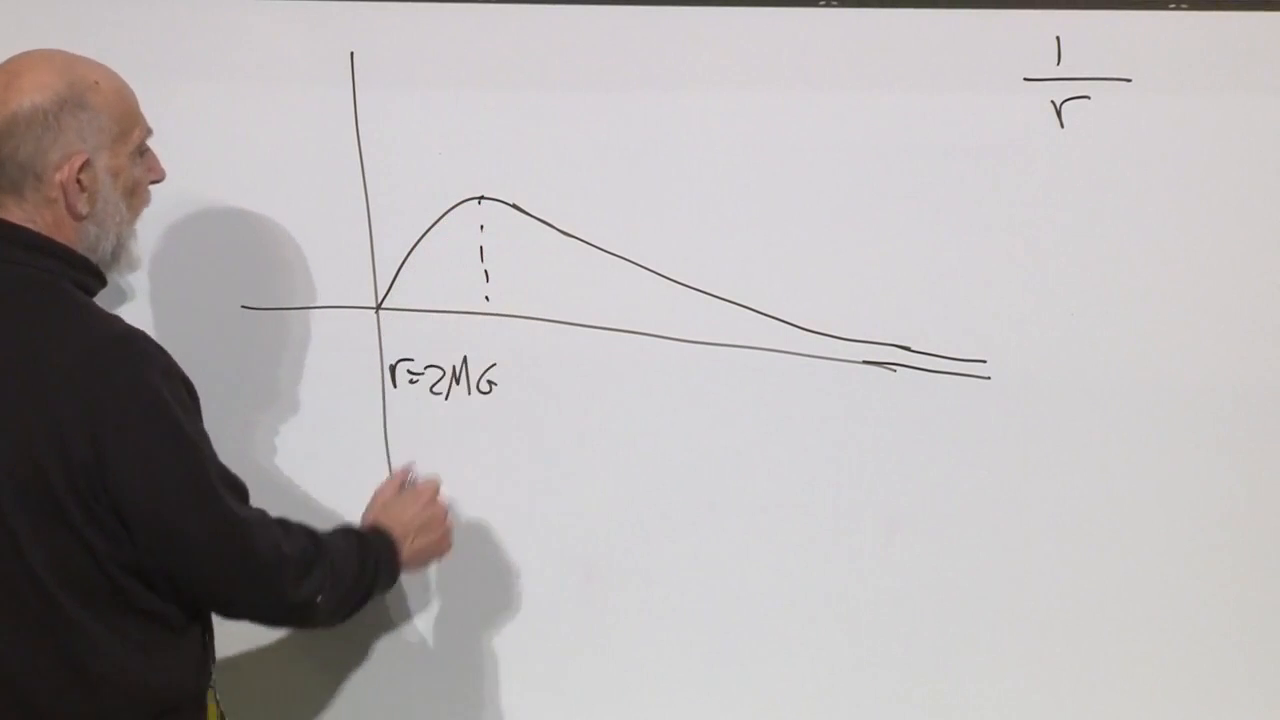
\includegraphics[width=0.88\textwidth]{lecture_06_figure_05.png}
\caption{光子エネルギーにおける動径因子。それは事象の地平面でゼロになり、大きな半径ではゼロに向かって減少し、その間に一つの極大を持つ。}
\lectureframe{00:50:50}
\end{figure}

\(L\)を固定したとき、動径方向の平衡は停留点を要求する。
\begin{equation}
\frac{d}{dr}
\left[
\frac{\sqrt{1-\frac{2MG}{r}}}{r}
\right]=0.
\end{equation}
微分すると、
\begin{equation}
-\frac{\sqrt{1-\frac{2MG}{r}}}{r^{2}}
+
\frac{MG}
{r^{3}\sqrt{1-\frac{2MG}{r}}}
=0,
\end{equation}
となり、したがって
\begin{equation}
r=3MG.
\label{eq:l6-photon-sphere}
\end{equation}
となる。この半径はシュヴァルツシルト半径の1.5倍である。通常、光子球と呼ばれる。

この停留点は極大であるため、円形光子軌道は不安定である。光子がちょうど\(3MG\)に置かれれば、そこにとどまる。任意に小さな動径方向の変位は、最終的にそれを極大から遠ざける。光子球のすぐ外側では、光線は脱出する前に非常に大きな角度を掃き、おそらくはブラックホールの周りを何度も巻くことができる。そのすぐ内側では、ほぼ接線方向の光線は何度か巻いた後、事象の地平面を通り抜けて落ち込むことができる。

\begin{figure}[htbp]
\centering
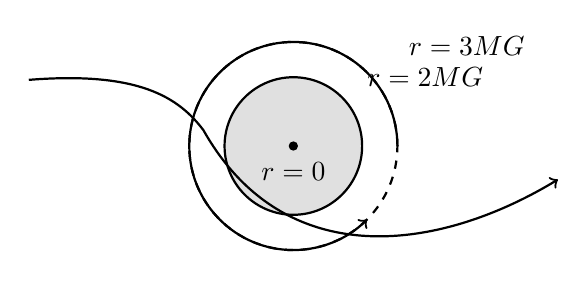
\begin{tikzpicture}[scale=1.12]
\fill[black!12] (0,0) circle (0.78);
\draw[thick] (0,0) circle (0.78);
\draw[dashed,thick] (0,0) circle (1.18);
\fill (0,0) circle (1.5pt);
\draw[->,thick] (1.18,0) arc (0:315:1.18);
\draw[->,thick] (-3.0,0.75)
  .. controls (-1.75,0.85) and (-1.30,0.55) .. (-1.02,0.18)
  .. controls (-0.10,-1.45) and (1.65,-1.20) .. (3.0,-0.38);
\node[right] at (0.73,0.78) {\(r=2MG\)};
\node[right] at (1.20,1.13) {\(r=3MG\)};
\node[below] at (0,-0.08) {\(r=0\)};
\end{tikzpicture}
\caption{事象の地平面、光子球、そして強く偏向された光線。不安定な円軌道に任意に近い光線は、脱出するか内側へ落ち込む前に、任意に大きな偏向を蓄積することができる。}
\end{figure}

\begin{classroomqa}
\audiencequestion{なぜ角運動量を固定するのか、またそれは光子の振動数や入射軌道とどう関係するのか。}
\lecturerresponse{各光線はブラックホールのまわりで保存される角運動量を運ぶ。その振動数は線形運動量の大きさを定め、中心からのずれは\(L\)の決定に寄与する。円軌道から離れていれば、半径と角運動量は独立に選べる。光子の円軌道を要求することは、その運動を唯一の半径\(3MG\)に結びつけ、式~\eqref{eq:l6-photon-energy}の因数分解はこの半径が\(L\)の大きさに依存しないことを示す。
\lecturetimestamp{00:54:43--00:57:02}}
\end{classroomqa}

\begin{classroomqa}
\audiencequestion{なぜエネルギーの極大が軌道を特定するのか。}
\lecturerresponse{\(L\)を固定して角運動を消去した後、残った関数は有効動径エネルギーの役割を果たす。停留点は動径方向の平衡を与える。極小なら安定であるが、この点は極大であり、したがって不安定な円軌道を与える。それを平衡であり同時に不安定であると呼んでも矛盾はない。
\lecturetimestamp{00:57:51--00:58:54}}
\end{classroomqa}

質量をもつ粒子は\(3MG\)の外側に時間的円軌道をもちうるが、光子球に最も近いそれらは不安定である。質量のない粒子は\(3MG\)における円軌道のみをもつ。光子球の内側では、接線方向に運動する光子は内向きに落ちる。より遅く運動する物体がそのような軌道を維持する見込みがより良いわけではない。この記述は角運動に関するものである。事象の地平面の外側では、十分外向きの光線は、その出発半径が\(3MG\)より下であってもなお脱出しうる。

\section{ブラックホールが像に及ぼす効果}

光子球は、ブラックホールが、他の点では変わらない空に貼り付けられた単なる暗い円盤ではない理由を説明する。背景天体からの光は複数の経路に沿って観測者に到達しうる。ある光線は穴の一方の側を通り、別の光線は反対側を通り、さらに別の光線は穴のまわりを1回以上周りうる。その結果には、ずれた像、重複した像、環、および追加の巻き付きに対応する、ますます細かくますます暗い像の無限列が含まれうる。正確な像は複雑であるが、その起源はすでに不安定軌道に含まれている。

光源、レンズ、観測者が十分に整列しているとき、像はアインシュタイン環を形成しうる。重力レンズ環は自然界で観測されている。完全なブラックホール像を得るには、多くの初期方向について零測地線を積分する必要があり、これはコンピュータに適した計算である。

\begin{classroomqa}
\audiencequestion{この光学的境界は光子球を指すのか、それとも地平面を指すのか。}
\lecturerresponse{それらは異なる役割を果たす。\(2MG\)における地平面は因果的境界であり、その内側から未来向きの信号は脱出しない。\(3MG\)における光子球は接線方向の運動と強いレンズ効果を支配する。二つの半径の間では、外向きの動径光線は脱出しうるが、接線方向の光線は落ち込む。中間の方向は脱出または捕獲の前にループしうる。
\lecturetimestamp{01:02:47--01:03:40}}
\end{classroomqa}

\begin{classroomqa}
\audiencequestion{一般的な光の経路は、単に描くだけでなく計算できるのか。}
\lecturerresponse{できる。零条件を測地線方程式またはEuler--Lagrange方程式に代入し、選んだ初期データで積分すればよい。方程式は概念的には新しいものではないが、光線追跡は代数的に煩雑であり、そのため数値計算が像を得る実用的な方法となる。
\lecturetimestamp{01:03:48--01:04:27}}
\end{classroomqa}

\begin{classroomqa}
\audiencequestion{Euler--Lagrange方程式を直接適用した方が円軌道の計算は難しくなっただろうか。}
\lecturerresponse{同じ結果を与えるだろう。作用はどちらの方法でも適切な出発点であるが、循環座標が保存エネルギーと角運動量を露わにする。それらの定数を先に用いることが円軌道条件への短い道である。
\lecturetimestamp{01:04:33--01:05:49}}
\end{classroomqa}

\section{地平面近傍の計量はRindler空間である}

ここで地平面に戻る。Schwarzschild係数はそこで発散するか消えるように見え、地平面を横切るときにそれらの符号は入れ替わる。それでも落下する観測者はその面で発散する局所曲率に出会わない。等価原理は、両方の記述がどのようにして真でありうるかを教えてくれる。

二次元Minkowski時空から始める。
\begin{equation}
d\tau^{2}=dT^{2}-dX^{2}.
\end{equation}
右Rindler楔において定義する。
\begin{equation}
X=\rho\cosh\omega,
\qquad
T=\rho\sinh\omega.
\label{eq:l6-rindler-map}
\end{equation}
\(\rho\)が一定の曲線は
\begin{equation}
X^{2}-T^{2}=\rho^{2},
\end{equation}
を満たすので、それらは双曲線であり、一様加速観測者の世界線である。式~\eqref{eq:l6-rindler-map}を平坦計量に代入すると
\begin{equation}
d\tau^{2}
=\rho^{2}d\omega^{2}-d\rho^{2}.
\label{eq:l6-rindler-metric}
\end{equation}
が得られる。ここで
\begin{equation}
\rho^{2}=4\xi,
\qquad
\omega=\frac{t}{2}.
\label{eq:l6-rindler-rescale}
\end{equation}
と置く。\(d\rho^{2}=d\xi^{2}/\xi\)であるから、式~\eqref{eq:l6-rindler-metric}は
\begin{equation}
d\tau^{2}
=\xi\,dt^{2}-\frac{d\xi^{2}}{\xi}.
\label{eq:l6-xi-metric}
\end{equation}
となる。

\begin{classroomqa}
\audiencequestion{角度座標すなわち横方向の座標はどこへ行ったのか。}
\lecturerresponse{それらは単に省略されているだけである。我々は地平線を横切る振る舞いを含む局所的な
\(t\)-\(r\) 平面を調べている。二つの
横方向は依然として正則であり、復元することができる。それらは解析している座標特異点を変えない。
\lecturetimestamp{01:16:27--01:16:47}}
\end{classroomqa}

Schwarzschild と比較するために、\(2MG=1\) となる単位を選ぶ。式~\eqref{eq:l6-schwarzschild}の動径部分は
\begin{equation}
d\tau^{2}
=
\frac{r-1}{r}\,dt^{2}
-
\frac{r}{r-1}\,dr^{2}.
\end{equation}
\(r=1\) のごく近くでは、小さな分子 \(r-1\) を保持しなければならないが、それ以外では無害な \(r\) の因子は 1 で置き換えてよい。したがって
\begin{equation}
d\tau^{2}
\simeq
(r-1)\,dt^{2}
-
\frac{dr^{2}}{r-1}.
\end{equation}
ここで
\begin{equation}
\xi=r-1,
\end{equation}
とすると、これはちょうど式~\eqref{eq:l6-xi-metric}である。地平線近傍の Schwarzschild
幾何は、局所的には平坦時空の Rindler 記述である。

\begin{classroomqa}
\audiencequestion{基礎となる時空が平坦であるのに、なぜこれらが加速座標でありうるのか。}
\lecturerresponse{加速度は観測者に属するものであり、必ずしも曲率に属するものではない。\(\rho\) を固定した世界線は
Minkowski 時空において一様に加速されている。同様に、ブラックホール近傍で固定された半径に保持される観測者は、自由落下に対して支えられていなければならない。等価原理により、完全な Schwarzschild
時空が曲がっているにもかかわらず、局所的な記述は一致する。
\lecturetimestamp{01:22:19--01:24:06}}
\end{classroomqa}

\section{Rindler 地平線の横断}

右ウェッジの公式は \(\xi>0\) のみを覆う：
\begin{equation}
X=2\sqrt{\xi}\cosh\frac{t}{2},
\qquad
T=2\sqrt{\xi}\sinh\frac{t}{2}.
\label{eq:l6-rindler-outside}
\end{equation}
曲面 \(\xi=0\) はヌル線 \(X=T\) である。未来ウェッジへと続けるために、
\begin{equation}
\zeta=-\xi>0
\end{equation}
とし、双曲線の役割を入れ替える：
\begin{equation}
T=2\sqrt{\zeta}\cosh\frac{t}{2},
\qquad
X=2\sqrt{\zeta}\sinh\frac{t}{2}.
\label{eq:l6-rindler-inside}
\end{equation}
計量は依然として
\begin{equation}
d\tau^{2}
=\xi\,dt^{2}-\frac{d\xi^{2}}{\xi},
\end{equation}
であるが、\(\xi<0\) のとき、\(dt^{2}\) の係数は負であり、\(d\xi^{2}\) の係数は正である。座標 \(\xi\)、したがって
Schwarzschild 動径方向は時間的となった；\(t\) は空間的となった。

\begin{figure}[htbp]
\centering
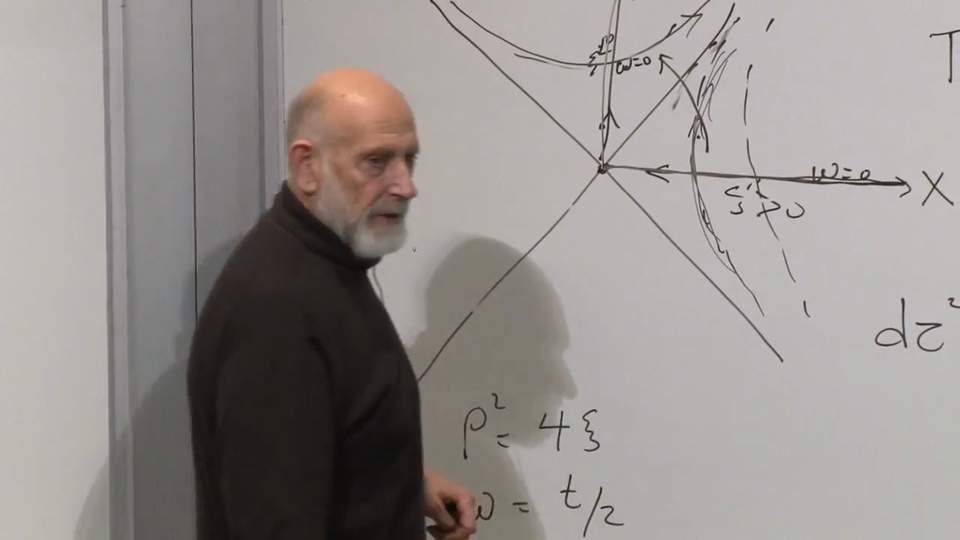
\includegraphics[width=0.88\textwidth]{lecture_06_figure_06.png}
\caption{Rindler ウェッジ、それらのヌル境界、および
\(\xi>0\) から \(\xi<0\) への継続。板書には
\(\rho^{2}=4\xi\) と \(\omega=t/2\) も記録されている。}
\lectureframe{01:29:40}
\end{figure}

\begin{classroomqa}
\audiencequestion{この座標図においていくつかの曲線は光より速く動くのか。}
\lecturerresponse{座標格子線は物質的物体の世界線である必要はない。その座標傾きは因果律に違反することなく超光速に見えることがある。物理的な光線はヌル線上にとどまり、物理的な粒子はそれらの局所的な光円錐の内側にとどまる。
\lecturetimestamp{01:28:44--01:29:08}}
\end{classroomqa}

Schwarzschild 内部へさらに進み続けると、最終的に
\(r=0\) に到達する。その境界は空間的である。したがってそれは場所というよりも時間として記述する方がよい：ブラックホール内部におけるすべての未来向きの時間的またはヌル的軌道はそこに到達する。場所を回り込むことはできる。自分の未来を回り込むことはできない。

\begin{classroomqa}
\audiencequestion{図は単に \(r=0\) を通って負の \(r\) へと続くことができるのか、そして \(r=0\) は依然として中心なのか。}
\lecturerresponse{座標図は線を延長するよう我々を誘うかもしれないが、古典的な Schwarzschild 解は曲率特異点で終わる。
\(r=0\) は依然として中心と呼ばれるかもしれないが、それは非常に異常な中心である：内部ではそれは空間的な未来境界である。そこを通って負の半径の領域へと至る正則な通り道は存在しない。
\lecturetimestamp{01:32:16--01:34:06}}
\end{classroomqa}

\begin{classroomqa}
\audiencequestion{Rindler 図における対角軸はヌル的か、そして落下する者は加速時間の有限の値で入ることができるのか。}
\lecturerresponse{はい、ウェッジの境界はヌル線である。自由落下する世界線はそのような線を通常の有限な事象において、有限な固有時間で横切る。加速座標 \(t\)、あるいは同等に
\(\omega\) は、外部の定 \(\rho\) 記述に沿って非有界に走る；無限になるのはその座標の割り当てであり、横断事象ではない。
\lecturetimestamp{01:34:26--01:35:03}}
\end{classroomqa}

\section{外側の Alice と落下する Bob}

Alice は重力に対して支えられながら固定された半径で外側にとどまり、Bob は自由落下するとしよう。地平線近傍で、Alice は Rindler 的な双曲線に従う。彼女の定 \(t\) スライスはヌル境界へとますます近づいて密集する。Alice が有限の \(t\) でラベル付けする Bob の世界線上のすべての事象は地平線の外側にあり、したがって彼女は彼の横断に有限の Schwarzschild 時間を割り当てることはない。

Bob は固有時間時計を携帯している。彼の軌道はその時計の有限な間隔でヌル線を横切る。彼が横切るとき、局所的に発散するものは何も起こらない。地平線は大域的に決定的であるが、局所的には通常である。

\begin{figure}[htbp]
\centering
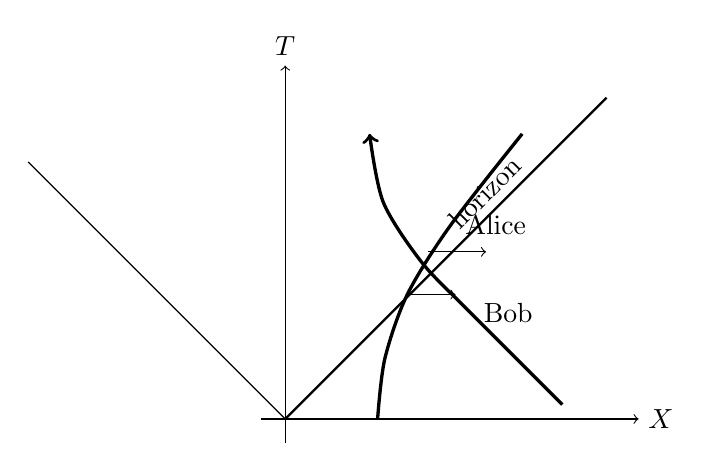
\begin{tikzpicture}[scale=1.02]
\draw[->] (-0.3,0) -- (4.4,0) node[right] {\(X\)};
\draw[->] (0,-0.3) -- (0,4.4) node[above] {\(T\)};
\draw[thick] (0,0) -- (4.0,4.0);
\draw[thin] (0,0) -- (-3.2,3.2);
\node[rotate=45,above] at (2.65,2.65) {horizon};
\draw[very thick]
  plot[smooth] coordinates {(1.15,0.0) (1.24,0.75) (1.52,1.55)
  (2.05,2.40) (2.95,3.55)};
\node[right] at (2.12,2.42) {Alice};
\draw[very thick,->]
  plot[smooth] coordinates {(3.45,0.18) (2.85,0.78) (2.25,1.38)
  (1.70,1.95) (1.22,2.70) (1.05,3.55)};
\node[right] at (2.35,1.32) {Bob};
\draw[->] (1.52,1.55) -- (2.12,1.55);
\draw[->] (1.78,2.08) -- (2.50,2.08);
\end{tikzpicture}
\caption{Alice の加速された外部世界線と Bob の自由落下世界線。Alice の座標スライスは地平線に近づく；Bob は有限な固有時間でそれを横切る。}
\end{figure}

\begin{classroomqa}
\audiencequestion{ボブが振り返ってアリスを見たとき、彼には何が見えるのか、また地平線を越えた後、彼の時計はどうなるのか。}
\lecturerresponse{ボブには、アリスが外側にとどまるために必要な加速度で後退していくのが見えるが、自分が越える瞬間に特異な事象が起こるのを見るわけではない。アリスは固定された半径に支えられていてもよい。軌道は別の可能な設定である。ボブの時計は、通常どおり彼の固有時\(\tau\)を測り続ける。内部で動径座標が時間的であると言うのは、因果的幾何を記述しているのであって、彼の腕時計が文字どおり物差しに変わるわけではない。彼の世界線は最終的に\(r=0\)で終わる。
\lecturetimestamp{01:39:51--01:44:45}}
\end{classroomqa}

このヌル線は、もはや座標係数が異常な振る舞いをする一つの点ではなく、地平線そのものとして認識される。その外側では、動径方向の光線のある族が外向きに進む。その内側では、未来光円錐の両方向がより小さい\(r\)へ向かう。未来向きの質量をもつ軌道はすべて、それらヌル方向の間に留まらなければならず、したがって特異点に到達する。

\section{信号、赤方偏移、そして形成されつつある地平線}

崩壊する物質が規則的な光パルスの列を放出するとしよう。遠方の観測者は、後のパルスをますます長い間隔で受け取る。それらの振動数は、可視光から赤外線、マイクロ波、電波へと移り、さらに長い波長へとずれていく。理想化された古典的計算では、外側の観測者は、地平線に近づく物質にますます後の信号を対応づけ続けることができるが、実際には光源は急速に赤くなりすぎ、暗くなりすぎて検出できなくなる。

\begin{classroomqa}
\audiencequestion{崩壊の間、外側の観測者には、すべての物質が地平線で単に凍りつくように見えるのか。}
\lecturerresponse{シュヴァルツシルト時間では、崩壊する物質の表面は地平線に漸近的に近づき、ますます凍りついたように見える。実際に観測されるものは光信号に符号化されており、それらの信号はますます遅延し、赤方偏移し、暗くなる。この座標による説明は、落下する物質が無限の固有時を経験すると述べているわけではない。
\lecturetimestamp{01:47:06--01:48:11}}
\end{classroomqa}

\begin{classroomqa}
\audiencequestion{十分に遅い観測者なら、落下の全歴史を復元できるのか。}
\lecturerresponse{放出され、観測者に到達することに成功した信号を通じてのみである。連続するパルスはますます離れ、赤方偏移する。感度に制限のない理想的な観測者なら、古典的信号をますます長い波長まで追うことができるが、実際の観測者には物体が薄れて見えなくなる。
\lecturetimestamp{01:48:13--01:52:00}}
\end{classroomqa}

\begin{classroomqa}
\audiencequestion{特異点が場所ではなく時間であると言うとき、正確には何を意味するのか。}
\lecturerresponse{\(r=0\)面は空間的である。いったん地平線の内側に入れば、未来向きの時間的またはヌル曲線はすべてそこで終わる。空間的な位置は別の経路を選ぶことで避けられるが、未来向きの世界線に沿って進み続ける限り、未来の境界は避けられない。
\lecturetimestamp{01:52:02--01:53:10}}
\end{classroomqa}

では、外側の観測者が物質の横断を決して見ないのなら、どうしてブラックホールは形成されたり質量を増やしたりできるのか。崩壊する球対称殻を考えよう。大域的地平線は、一つの固定された半径に前もって存在する物質面として待っているのではない。それは中心から始まり外側へ成長し、ブラックホール領域が形成されるにつれて崩壊する殻と出会う。外部のシュヴァルツシルト記述では、依然として殻は最終的な地平線に漸近的に近づく。地平線が大域的にどのように位置づけられるかを含む完全な時空像は、次の講義の主題である。

\begin{figure}[htbp]
\centering
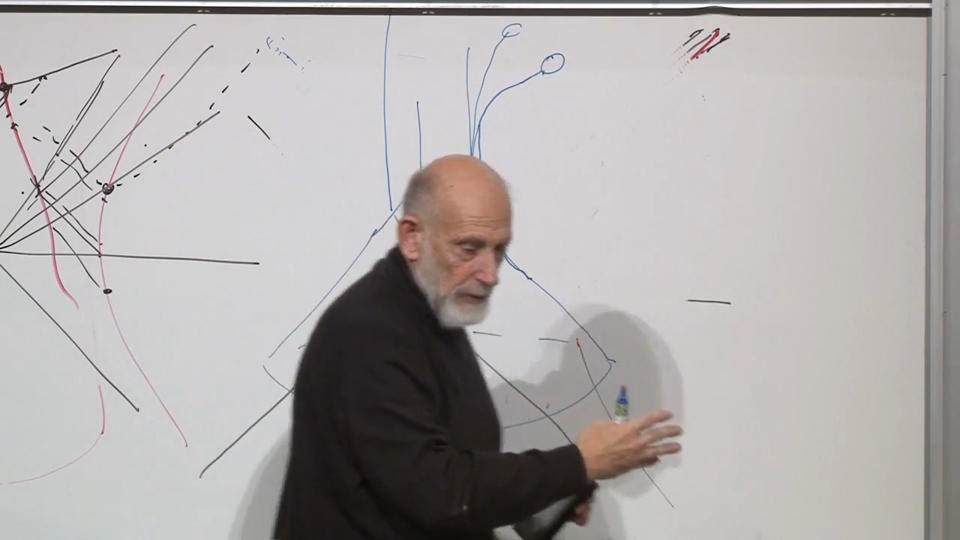
\includegraphics[width=0.90\textwidth]{lecture_06_figure_07.png}
\caption{崩壊する殻と、中心から外側へ成長してそれと出会う地平線。この図は、次の講義で展開される大域的崩壊幾何の予告である。}
\lectureframe{01:57:25}
\end{figure}

\begin{classroomqa}
\audiencequestion{外部座標時間で何も地平線を横切らないのなら、どうしてブラックホールは形成されたり成長したりできるのか。}
\lecturerresponse{その前提は、座標に関する記述と大域的な記述を混同している。崩壊する物質は有限の固有時で関連する領域に到達する一方、事象の地平線は時空全体の因果構造によって決まる。殻の描像では、それは中心から始まり外側へ成長して殻と出会う。外側の観測者による遅延し赤方偏移した見え方は、その大域的地平線と依然として整合している。
\lecturetimestamp{01:53:11--01:57:34}}
\end{classroomqa}

\section{二つの球の間の脱出方向}

地平線と光子球は、光線の問題を別々の場合に分ける。半径
\begin{equation}
2MG<r<3MG,
\end{equation}
では、動径方向に外向きの光線は無限遠へ脱出できる。接線方向の光線は脱出できず、内側へ落ちる。それら方向の間には脱出円錐が存在する。地平線に近づくにつれ、その円錐は外向き動径方向の周りで狭くなる。地平線を越えた後、それは完全に閉じる。

\begin{classroomqa}
\audiencequestion{事象の地平面と光子球の間にある光源は、外側へ何らかの信号を送ることができるか。}
\lecturerresponse{できる。十分に動径的な外向きのヌル光線は、その放出事象が\(2MG\)の外側にある限り脱出する。\(3MG\)の内側では角運動が内向きに落ち込むという主張は、動径方向の脱出を禁じるものではない。結果は放出方向に依存し、光源が地平面に近づくにつれて許される外向き錐は狭くなる。
\lecturetimestamp{01:57:34--01:59:48}}
\end{classroomqa}

\begin{classroomqa}
\audiencequestion{外側から到来する光線は光子球の内側へ入り込み、向きを変えて再び出てくることができるか。}
\lecturerresponse{ここで議論しているタイプのヌル測地線に沿ってはできない。転回点では動径速度がゼロになるので、光線は\(3MG\)より小さい半径で一時的に接線方向になる。そこでは角方向の軌道は外向きに戻るのではなく内向きに落ち込む。しかし、すでに二つの球の間にある光源は、地平面を横切る前に十分に動径的な外向き光線を放出することができる。
\lecturetimestamp{01:59:49--02:01:27}}
\end{classroomqa}

最後の問いは意図的に未解決の度合いが高い。アリスとボブがともに地平面の外側の同じ半径に保持されていると想像しよう。近くの観測者どうしは明らかに信号を交換できる。彼らが球の周りで遠く離れている場合、直接のヌル経路とその限界角範囲を求めるには明示的な測地線計算が必要である。クラスは間接的な経路を提案する。すなわち、メッセージをほぼ動径方向に外側へ、より安全な半径にある中継点へ送り、そこで周囲を運び、再び内側へ送り返すのである。別の版では、外向きに投げられた物体または信号が向きを変えて戻ることを許す。これらの経路は、接線方向の円軌道が存在しないからといって、それだけで外部観測者間のあらゆる通信が禁じられるわけではない理由を示している。

\begin{classroomqa}
\audiencequestion{地平面近くの同じ半径に静止している二人の観測者は、ブラックホールの周りで通信できるか。}
\lecturerresponse{局所的には、できる。広く離れた、または正反対側にある観測者については、直接経路の限界は講義では導出されておらず、定理に格上げすべきではない。議論はまずその角方向測地線の問題を未解決のままにし、次に間接的な信号がほぼ動径方向に外側へ進み、より大きな半径で周囲を中継され、戻ってくることができると述べる。地平面に近づくにつれて直接役立つ角範囲はますます狭くなるが、地平面の外側では外向きの経路が依然として利用可能である。
\lecturetimestamp{02:01:29--02:04:17}}
\end{classroomqa}

次の段階は、これらの地平面近傍の概略を、崩壊する物体の大域的な幾何学に置き換え、事象の地平面が正確にどのように成長するかを見ることである。
